\documentclass[11pt,a4paper]{article}
\usepackage{ifpdf}
\usepackage[utf8]{inputenc}
\usepackage[francais]{babel}
\usepackage[T1]{fontenc}
\usepackage[nottoc, notlof, notlot]{tocbibind}
\usepackage[unicode=true,pdftex,colorlinks=true,linkcolor=black,urlcolor=black,citecolor=black]{hyperref}
\usepackage{natbib}
\usepackage{graphicx}

\parindent 0.8cm
%\setlength{\parskip}{0.5em plus 0.2em minus 0.2em}

\title{Projet HADL}
\author{Anthony \textsc{Caillaud} Manoël \textsc{Fortun}}
\date{\today}
\ifpdf
\pdfinfo {
/Author (Anthony Caillaud Manoël Fortun)
/Title (Projet HADL)
/Subject (Projet HADL)
/Keywords ()
/CreationDate (D:20100329212218)
}
\fi


\begin{document}

\maketitle


\clearpage
\tableofcontents
\clearpage
\section{Introduction}

Dans le cadre de notre module Composants dans lequel nous avons pu étudier les
modèles à composants et leurs fonctionnements, nous avons du modéliser et écrire
notre propre langage d'architecture logicielle à composants. Ce projet ne
consistait pas seulement en la définition d'un langage d'architecture à
composants, mais aussi en l'implémentation en langage objet d'un moteur
d'architecture à composants. Ce rapport présente donc le travail que nous avons
pu effectuer sur cet HADL(home architecture definition langage). Dans un
premier temps, le travail de modélisation des concepts composants
(meta-modélisation) ainsi que l'implémentation du modèle vous sera présenté.
Ensuite, l'application du modèle à composants (modélisation) vous sera
expliquée à travers l'exemple du système Client/Serveur. Enfin, nous
détaillerons le meta-meta-modèle que nous avons pu définir pour notre HADL.


 
\section{Description du méta-modèle HADL}
\subsection{Définitions}
L'architecture logicielle à base de composants est consitutés de trois
principaux éléments : des composants, des configurations et des connecteurs.\\

\subsubsection{Eléments principaux}

% - Def Composant
 Un composant est une unité de composition qui spécifie une ou plusieurs
 fonctionnalités. Celui-ci peut être déployé indépendemment, il s'agit de la
 brique élémentaire.\\

%- Def Configuration
Une configuration est un ensemble de composants et de connecteurs, il définit la
façon dont ils sont reliés entre eux. Cette unité de l'architecture logicielle
à base de composants est nécessaire aux bonnes liaisons entre composants. Elle
permet de savoir si ces liaisons relatives aux connecteurs permettent une
communication correcte. C'est la configuration qui gère tous les composants et
tous les connecteurs qui la composent.\\

%- Def Connecteur
Un connecteur explicite est une unité effectuant une liaison entre des
composants ou des configurations. Les connections proprement dites s'effectuent
grâce à des Rôles (Rôles From et Rôles To) et une ''Glue'' qui représente la
fonction modifiant les informations transférées. Il peut être comparé à un
adaptateur entre deux composants.\\

\subsubsection{Eléments secondaires}

%-Def Interface 
L'interface d'un composant, connecteur ou configuration est l'ensemble des
éléments fournis pour l'intéraction avec le composant, connecteur ou
configuration. Il s'agit plus d'un concept que d'un élément concret. Une
interface est généralement constituée de ports et de services.\\

%- Def Port
Un port est un point d'entrée ou de sortie d'un composant ou configuration, il
pourrait s'apparenter à un attribut d'une classe si on fait le rapprochement
entre le modèle composant et le modèle objet.\\

%- Def  Service
Un service est une opération disponible auprès d'un composant, il y a des
services fournis par un composant et des services requis pour son fonctionnement.
Un service peut être assimilé à une méthode toujours dans le parallèle
composant/objet. Un service peut être relié à des ports ce qui signifie que
certains ports seraient les entrées du service et d'autres ports seraient la ou
les sorties du service.\\

%-Def Propriétés
Les propriétés sont des éléments appartenant aux configurations ou composants,
les propriétés peuvent définir une particulatité du comportement ou un élément
dont on peut se servir, comme un attribut de classe.\\

%-Def Contraintes
Les contraintes sont des éléments importants, puisque elles définissent ce dont
ont besoin les composants ou configurations pour fonctionner,  par exemple la
présence d'une librairie particulière.\\

%-Def Roles
Ce concept est propre aux connecteurs, il y a les roles from et role to qui
constituent l'interface des connecteurs, leurs entrées et leurs sorties.\\

%-Def Lien
Les liens sont des éléments qui permettent de relier des composant entre eux, ou
une configuration à un composant. On distinguera deux types de liens:
\begin{itemize}
  \item Les attachements qui sont des liens entre composants, lien qui inclut un
connecteur,
  \item Les bindings qui relient les ports de configuration aux port de
  composant, lien qui n'inclut pas de connecteur.
\end{itemize}
 
\subsection{Analyse}

Lien= attachement= binding= connecteur

port service

Parler des fonctions utile




\subsection{Diagrammes}

diagramme de l'implémentation

Quelques explications



\clearpage
\section{Description du système Client/Serveur}
\subsection{Définitions}
Le système Client/Serveur est une bonne représentation au niveau M1 d'une
architecture logicielle à composants. En effet, chacune des partie constituant
ce système peut être vu comme un composant faisant partie d'une configuration
représentant celui-ci. Ces trois composants principaux sont le client, le
serveur et le connecteur RPC qui permet la communication entre les deux
premières entités.\\

Le client est donc un simple composant de la configuration ''Client/Serveur''
permettant l'envoi et la réception de messages. Le serveur, quant à lui, est
une configuration comprenant plusieurs autres composants permettant le
traitement du message reçu.


\subsection{Analyse}
Au niveau M1, chacun des composants offre des services. Tout d'abord, le
client permet donc d'envoyer et de recevoir des messages. Ces deux services
sont liés à deux ports différents.\\


Les trois composants de la configuration ''Serveur'' sont ConnectionManager,
SecurityDB et Database.
 
ConnectionManager est le composant qui va recevoir en premier le message envoyé
par le client. En effet, via un lien Binding, c'est ce composant qui communique
avec la configuration ''Serveur''. Dans notre implémentation, il propose deux
services indiquant l'entrée et la sortie du message dans le composant.

Le composant SecurityDB est celui qui effectue des vérifications liées à
la sécurité et aux autorisations concernant le message provenant du client.
Nous avons choisi de ne pas implémenter de sécurité pour les messages que nous
voulions faire circuler. Le composant affiche uniquement un message dans le
terminal signalant le passage du message dans celui-ci. 

Enfin, le composant Database représente la base de données interrogée. Pour
cela, nous avons mis en place une HashMap avec quelques entrées. Un service de
ce composant est de renvoyer la valeur contenu dans la Map correspondant à la
clé reçue.\\

Tous ces composants, qui forment le Serveur, sont reliés entre eux à l'aide de
connecteurs. Ces connecteurs sont donc au nombre de trois : ClearenceRequest,
SecurityQuery et SQLQuery. La Glue de chacun de ses connecteurs ne fait que
transmettre le message, aucune autre action n'est effectuée sur le message.

ClearenceRequest fait le lien entre les composants ConnectionManager et
SecurityDB. Quant à lui, le connecteur SecurityQuery relie SecurityDB et
Database. Enfin, SQLQuery permet aux composants ConnectionManager et Database
de communiquer.\\

RPC est lui aussi, comme les autres connecteurs décrits précédemment, un
connecteur dont la Glue n'effectue uniquement la transmission du message entre
le composant Client et la configuration Serveur.

\clearpage
\subsection{Diagrammes}

\begin{figure}[h]
  		\centering
  		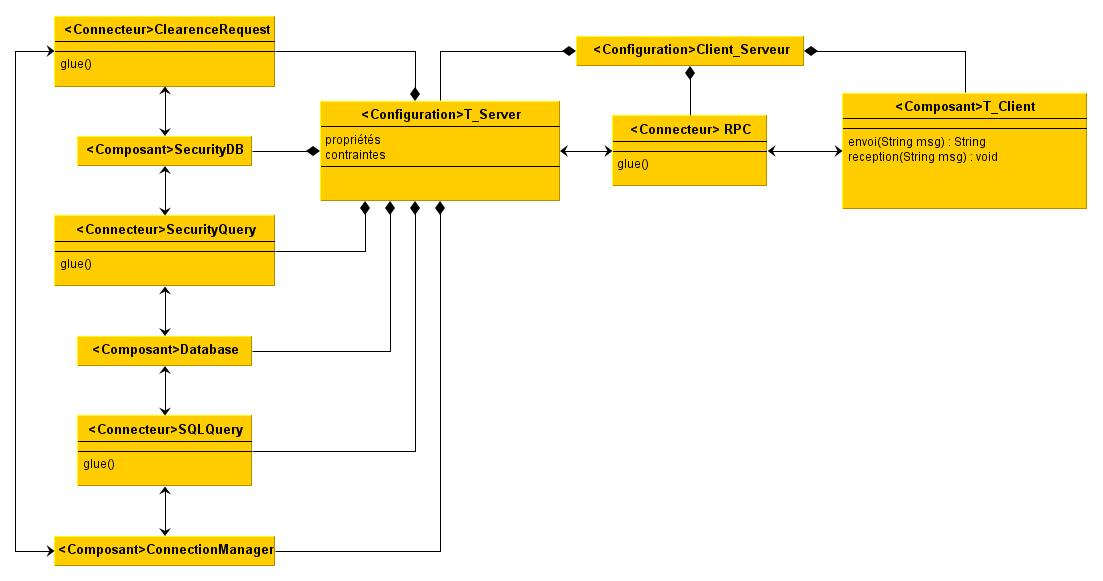
\includegraphics[height=14cm,width=15cm,angle=90]{M1.jpg}
  		\caption{Diagramme du système Client/Serveur}
  		\label{Diagramme du système Client/Serveur}
\end{figure}

\clearpage


\section{Description du méta-méta-modèle HADL}
\subsection{Définitions}
%- Def Meta-Entité
%- Def Meta-Relation
\subsection{Analyse}

Nous avons choisi pour ce méta-méta-modèle de ne pas inclure tous ce qui
concerne les ports, services et d'autres notions afin de ne pas surcharger le
diagramme. Ces notions omises au niveau M2 sont toutes des méta-entités.
\subsection{Diagrammes}

\begin{figure}[h]
  		\centering
  		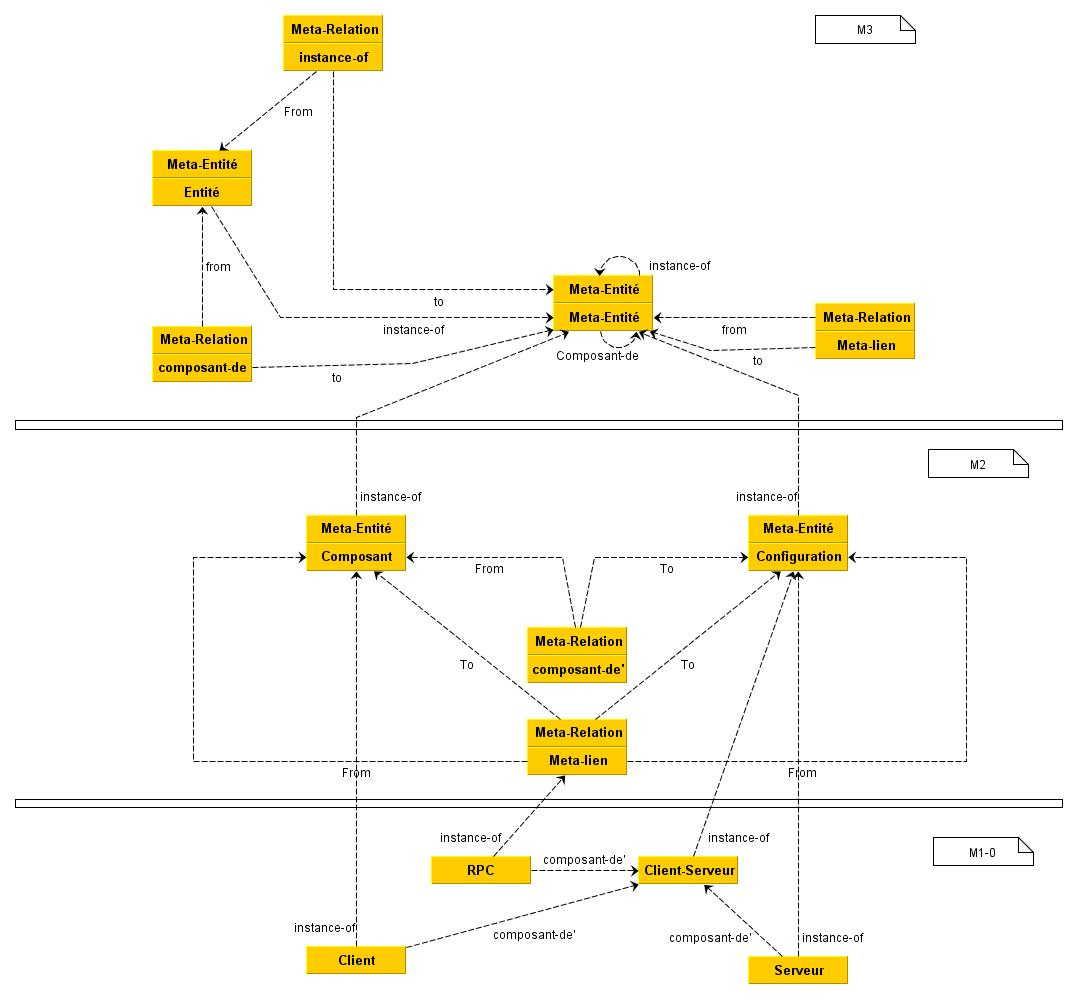
\includegraphics[height=14cm,width=15cm]{meta-meta-modele.jpg}
  		\caption{Diagramme du méta-méta-modèle HADL}
  		\label{Diagramme du méta-méta-modèle HADL}
\end{figure}


\section{Conclusion}

En conclusion, le travail effectué sur cet HADL nous a permis de bien observer
et de bien comprendre les différents niveaux d'une architecture logicielle à
composants. Ceci nous a permis de voir les différents niveaux d'abstraction
d'une architecture logicielle et ce qui les relient. De plus, l'implémentation
de la méta-modélisation jusqu'à l'instanciation nous a permis de voir
concrètement ces niveaux.


\end{document}
